\subsection{Valg af antal RC-led}
\label{ValgAfAntalRCLed}
2.62dB per 5dB volumen ændring
Vi startet med en figur der viser hældningerne ved 1,2,3,4 RC led, så kan vi komme ``så'' tæt på
så har vi et grundlag for hvorfor et led ikke er nok og hvorfor 4 er for meget
Hvad sker der hvis man har for mange led, hvad kan være negativt ved det? Vi ønsker at holde det simpelt og ``billigt'' 
Hvilke værdier har de forskellige RC-led
Vi fokuserer på 2 og 3 led
Udregninger i bilag, vis et eller to eksempler (for 1 og 2 RC-led) 
Kondensatorerne udvælges efter skøn (bedts muligt fit til kurven)

%Det egentlige afsnit starter her:
Dette afsnit har til formål at finde ud af hvor mange RC-led kredsløbet skal indeholde, svarende til hvor mange brøkdele dæmpningen skal deles op i fra $2.62dB$ til $0dB$.


Der ønskes et maksimalt gain på $2.62dB$, baseret på antagelser lavet i \fullref{ISO226}.
Som udgangspunkt dimensioneres $R_i$ til at være $10K\Omega$.
Gainet på $2.62dB$ omregnes til en gainfaktor:
\begin{equation}
	G_0 = 10^{\frac{2.62}{20}} = 1.3335
\end{equation}
\noindent
Dette er den maksimale forstærkning 



\subsection{1 RC-led}
Når vi regner med et RC-led, skal vi sikre at vi får en forstærkning på 1, svarende til 0dB. 
%
\begin{equation}
	G_1 = 1 = \frac{10K\Omega}{10K\Omega}
\end{equation}
\noindent
%
Så finder vi tilbagekoblingsmodstanden ved $G_1$
%
\begin{equation}
	R_f' = R_i*G_1 = 10K\Omega*1 = 10K\Omega
\end{equation}
\noindent
%
Så kan vi beregne $R_1$
%
\begin{equation}
	R_1 = \frac{R_f*R_f'}{R_f-R_f'} = \frac{13.335K\Omega*10K\Omega}{13.335K\Omega-10K\Omega} = 39.983K\Omega
\end{equation}
\noindent
%indsæt resten af formlerne for 2 og 3 led
Når alle gains er udregnet for 1-8 RC-led kan en kondensatorværdi estimeres ved at udregne værdien hvis man ønsker en knækfrekvens omkring $20 Hz$, dette kan gøres med følgende formel:
\begin{equation}
C_1=\frac{1}{R_1*2*\pi*f}
\end{equation}
Dette er for den første kondensatorværdi og resten kan forsøges at estimere, men da poler og nulpunkter risikerer at overlappe. (hvilket risikerer i stejlere og tidligere hældning)
Derfor kan det være svært at komme regne sig frem til den præcise værdi af $C$, simulering kan derfor være en bedre fremgangsmåde for at fastslå den endelige værdi af alle $C-ledene$. 
Udover at de enkelte poler kan overlappe er den generelt svært at estimere hvilken frekvens den næste pol skal ligge ved, (hvad skal fremgangsmåden være?)
Eftersom der ønskes en lineær hældning vil en lineær hældning for frekvensresponsen bestræbes der også et lineært forløb for afskæringsfrekvensen.

%indsæt udregningerne af logstep og dernæst C
%
\begin{figure}[H]
	\centering
	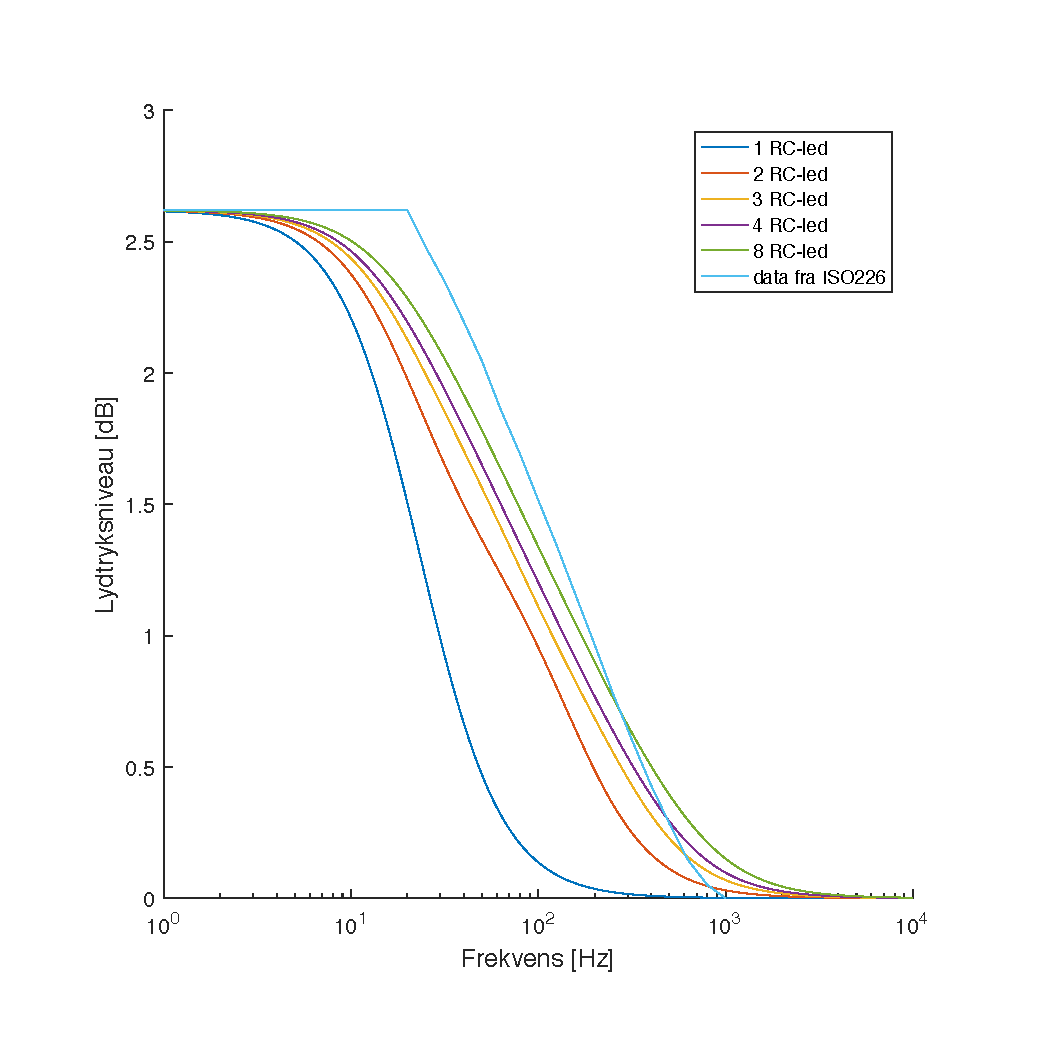
\includegraphics[resolution=300,width=\textwidth]{Figure/DesignAfFilter/1,2,3,4,8RC-ledGain2,62.pdf}
	\caption{Overføringsfunktion for filtre med henholdsvis 1,2,3,4 og 8 RC-led, hvor den logaritmiske x-akse angiver frekvens i hertz og den lineære y-akse angiver lydtryksniveau i dB.}
	\label{fig:1-8RC-ledIkkeJusteretC}
\end{figure}
\noindent
%
På \autoref{fig:1-8RC-ledIkkeJusteretC} illustreres den forskellige overføringsfunktioner for filtrene med et gain på $2.62 dB$ med tilhørende poler udregnet til $20 Hz$.
%Der er lavet flere forskellige plots som hver illustrer effekten af at tilføje flere led til filtret.
Der ønskes som sagt et så lineært forløb, mellem to punkter der henholdsvis har en forstærkning af signalet på $2.62 dB$ ved $20 Hz$ samt en forstærkning på $0 dB$ ved $1000 Hz$.
Filtret med 1 RC-led fravælges da det ikke har den tilsigtede hældning, det har en for stejl hældning.
Denne hældning kan ikke justeres da pol og nulpunkt parret kun kan flyttes ud ad x-aksen.
Filtret med 2 RC-led fravælges da det ikke har et lineært forløb efter indrulningsforløbet, men et mindre knæk opad på grafen omkring XX$1 dB$.
Derimod har filtret med 3 RC-led et meget lineært forløb uden betydelige knæk på grafen, samt en hældning der stemmer overens med det af den ønskede.
Funktionen knækker for tidligt i forhold til det ønskede, dette kompenseres der senere for med justering af hvor den første pol befinder sig.
Filtrene med 4 og 8 RC-led fravælges da det vurderes redundant at indføre unødige led, da de ønskede specifikationer kan opnås med færre komponenter, altså filtret med 3 RC-led.

Med dette vælges det derfor at udføre filtersystemet med et fraktalordensfilter der indeholder 3 RC-led.
Videre finjustering af filtrene med 3 RC-led foretages i \autoref{TilpasningAfFilter}.







%Her illustrerer knækkene tydeligt at afskæringsfrekvensen er for lav og videre justering bliver gjort manuelt i simuleringsprogrammet \textit{LTspice}.

%møde
%hvordan findes de andre C værdier
%Hvordan ved vi hvad der er godt nok
%Pænt nok= ingen krumninger over forløbet
%det er ok at simulere sig frem til C led (sofus har en udregningsmetode til at finde poler og nulpunkter)

%minus 2's kompliment


%pol(knæk nedad)
%nulpunkt(den retter ud)

%find forskrift med kvotienter
%find $r^2$